% \chapter{Corrosion of Steel in Reinforced Concrete Bridges}
\chapter{钢筋混凝土桥梁中的钢筋腐蚀}
\label{chp:corrosion-of-steel-rc-bridge}
% \section{Introduction}
\section{简介}
% This chapter of the Guide provides essential information for addressing corrosion of reinforcing steel in conventionally reinforced concrete structures. The focus is on controlling and mitigating corrosion for extended durability and service life. Corrosion in prestressed or posttensioned concrete structures is not discussed.
\bkn{指南}的这一章提供了解决传统钢筋混凝土结构中钢筋腐蚀问题的基本信息。重点是控制和减轻腐蚀,以延长耐用性和使用寿命。未讨论先张或后张预应力混凝土结构中钢筋/预应力钢材的腐蚀。

% The description of corrosion in \cref{sec:description-corrosion} covers the diffusion process that enables the penetration of chlorides through concrete and the creation of corrosion cells once the chlorides infiltrate. It also addresses the patchaccelerated corrosion commonly referred as “ring anode corrosion” in repairs. \cref{sec:factor-influencing-corrosion} describes factors influencing corrosion including chloride contamination and carbonation. \cref{sec:strategy-address-corrosion} provides a summary of strategies for addressing corrosion in new and existing structures; different levels of corrosion protection is considered, such as the corrosion prevention, corrosion control, corrosion passivation, and the electrochemical treatments. \cref{sec:case-study-addressing-corrosion} summarizes case studies that address corrosion in existing structures.
\cref{sec:description-corrosion} 中对腐蚀的描述涵盖了氯离子渗透混凝土的扩散过程,以及一旦氯离子渗透后腐蚀单元的产生过程。 它还解决了维修中通常称为“环形阳极腐蚀”的斑块加速腐蚀。\cref{sec:factor-influencing-corrosion}描述影响腐蚀的因素,包括氯离子污染和碳化。\cref{sec:strategy-address-corrosion}总结了解决新结构和现有结构腐蚀的策略;考虑了不同级别的腐蚀保护,例如腐蚀预防、腐蚀控制、腐蚀钝化和电化学处理。\cref{sec:case-study-addressing-corrosion}总结了解决现有结构腐蚀问题的案例研究。

% Faced with rising maintenance costs, many engineers and owners recognize the need to protect existing structures from future corrosion damage. As a result, the use of corrosion mitigation systems to delay the need for future concrete rehabilitation is increasing. Selecting the appropriate corrosion mitigation approach is based on many factors, including the amount and depth of contamination (chloride ingress or carbonation), amount of concrete cracking and concrete damage, severity and location of corrosion activity (localized or widespread), expected environmental exposure, use and service life of the structure, and the cost and design life of the corrosion protection system.
面对不断上涨的维护成本,许多工程师和业主认识到有必要保护现有结构免受未来的腐蚀破坏。 因此,越来越多地使用缓蚀系统来推迟未来混凝土修复的需求。 选择适当的腐蚀缓解方法基于许多因素,包括污染的数量和深度(氯离子渗透或碳化)、混凝土开裂和混凝土损坏的数量、腐蚀活动的严重程度和位置(局部或广泛)、预期的环境暴露、 结构的使用和使用寿命,防腐系统的成本和设计寿命。

% Deicing salts applied during winter months generally contain chlorides. Chloride solutions penetrate existing cracks and diffuse through the concrete cover to the reinforcing steel, initiating corrosion. Corrosion products exert stresses that can crack the concrete and cause delaminations and spalling.
冬季使用的除冰盐通常含有氯化物。 氯化物溶液渗透现有裂缝并通过混凝土保护层扩散到钢筋上,引发腐蚀。 腐蚀产物施加的应力会使混凝土开裂并导致分层和剥落。

% One approach to mitigating the problem is to prevent or minimize chloride penetration of chlorides by minimizing cracking using low permeability concretes, adequate concrete cover over the steel, membranes, sealers,or overlays. Another approach is to prevent the steel from corroding or to minimize the rate of corrosion through means such as the use of corrosion-resistant reinforcement or cathodic protection. Depending on the specifics of a project, one or a combination of both of these approaches may be desirable.
缓解该问题的一种方法是通过使用抗渗混凝土、在钢、膜、密封剂或保护层上覆盖足够的混凝土来最大程度地减少开裂,从而防止或最小化氯离子的渗透。 另一种方法是通过使用耐腐蚀钢筋或阴极保护等方式防止钢材腐蚀或将腐蚀速度降至最低。 根据项目的具体情况,可能需要这些方法中的一种或两种方法的组合。

% \section{Description of Corrosion}
\section{腐蚀的描述}
\label{sec:description-corrosion}
% \subsection{The Corrosion Process}
\subsection{腐蚀过程}
% The corrosion of steel in concrete is an electrochemical reaction similar to that of a battery. The corrosion rate is influenced by various factors including chloride-ion content, pH level, concrete permeability, and availability of moisture to conduct ions within the concrete. For corrosion to initiate in reinforced concrete, four elements are required to complete the corrosion cell: an anode, a cathode, ionic continuity between the anode and cathode through an electrolyte, and a metallic (electrical) connection between the anode and cathode.
钢材在混凝土中的腐蚀是一种类似于电池的电化学反应。腐蚀速率受多种因素影响,包括氯离子含量、pH 值、混凝土渗透性以及在混凝土内传导离子的水分可用性。要在钢筋混凝土中形成腐蚀,需要四个元素来完成腐蚀电池:阳极、阴极、阳极和阴极之间通过电解质的离子连续性,以及阳极和阴极之间的金属(电)连接。

% The anodic site becomes the site of visible oxidation (corrosion) and the cathode is the location of the reduction reaction which is driven by the activity at the anode. In reinforced concrete, the metallic path can be provided by the mild steel reinforcing or embedded prestressing strands. The ionic path is provided by the concrete matrix with sufficient moisture due to the permeability of concrete.
阳极位置是可见氧化(腐蚀)的位置,阴极是还原反应的位置,还原反应由阳极的活性驱动。在钢筋混凝土中,金属路径可以由低碳钢加固或嵌入的预应力钢绞线提供。由于混凝土的渗透性,离子路径由具有充足水分的混凝土基体提供。

% At the anode, iron is oxidized to ferrous ions:
在阳极,铁被氧化成亚铁离子:
\[ \ce{Fe -> Fe2+ + 2e-}\]

% At the cathode, a reduction reaction takes place. In an alkaline environment, the reduction reaction is typically:
在阴极则发生还原反应。在碱性环境中,还原反应通常是:
\[ \ce{ 2H2O + O2 + 4e- -> 4OH- } \]

% For the corrosion process to be initiated, the passive oxide film on the reinforcing steel must be broken. In most cases this is due to the presence of sufficient quantities of chloride ions in the concrete matrix at the level of the steel. Chloride-induced corrosion is most commonly observed in structures exposed to roadway deicing salts or in marine environments with direct exposure to salt water or wind-borne sea spray. Chlorides can also be introduced to the concrete during the original construction by the use of contaminated aggregates, water, or chloride-containing admixtures.
为了启动腐蚀过程,必须破坏钢筋上的钝化氧化膜。在大多数情况下,这是由于在钢筋所在位置的混凝土基体中存在足够数量的氯离子。氯离子引起的腐蚀最常见于暴露于道路除冰盐的结构或直接暴露于盐水或风浪的海洋环境中。在最初的施工过程中,通过使用受污染的骨料、水或含氯化物的外加剂,氯离子也可能被引入混凝土中。

% Over time, the corroding area (anode) will become more acidic as hydroxyl ions (\ce{OH-}) are consumed from the concrete in contact with the corroding area, and the cathode will become more alkaline by the generation of hydroxyl ions (\ce{OH-}).
随着时间的推移,腐蚀区域(阳极)将变得更加酸性,因为氢氧根离子(\ce{OH-})从与腐蚀区域接触的混凝土中被消耗掉,而阴极将通过产生氢氧根离子而变得更加碱性( \ce{OH-})。

% \subsection{The Diffusion Process}
\subsection{扩散过程}
% To the casual observer, uncracked concrete is a solid and impenetrable material. Viewed under a microscope, however, concrete is a labyrinth of fine capillaries, pores and voids between the individual cement and aggregate particles. The degree of porosity depends on the quality and density of the concrete mix.
对于不经意的观察者来说,未开裂的混凝土是一种坚固且坚不可摧的材料。然而,在显微镜下观察,混凝土是单个水泥和骨料颗粒之间的细毛细管、孔隙和空隙的迷宫。孔隙度取决于混凝土混合料的质量和密度。

% Due to this porosity, liquids can soak into the exposed surfaces of the concrete and carry contaminants such as chloride ions with them. Over time, the concentration of chloride ions within the concrete will tend to equalize as governed by Fick's Law.
由于这种孔隙率,液体会渗入混凝土的裸露表面,并携带氯离子等污染物。随着时间的推移,受菲克定律的支配,混凝土中氯离子的浓度将趋于平衡。

% In a one-dimensional case, Fick's Law can be expressed and illustrated as follows;
在一维情况下,菲克定律可以表达如下:
\begin{equation}
  \label{eq:fick-law-one-dimensional}
  C(x.t) = C_0 \left( 1-\erf \frac{x}{2\sqrt{D_\text{c}t}}\right)
\end{equation}
\begin{EqDesc}{C(x.t)}
  \item[C(x,t)] 深度 $x$ 处在时间 $t$ 时的氯离子浓度;
  \item[C_0] 表明氯离子浓度(\unit{kg/m^3});
  \item[D_\text{c}] 氯离子扩散常数(\unit{cm^2/yr});
  \item[\erf] 误差函数(来自标准数学表)。
\end{EqDesc}

% This expression indicates that the chloride concentration within the concrete will tend to equalize with the chloride concentration exposed to the surface over time. As expected, the chloride concentration within the concrete is greater near the exposed surface and increases with time at any point within the concrete. Concrete with a lower chloride diffusion constant (Dc) will provide longer term protection to reinforcing steel located at depth x from the surface of the concrete.
该表达式表明,随着时间的推移,混凝土中的氯离子浓度将趋于与暴露于表面的氯离子浓度相等。正如预期的那样,混凝土中的氯离子浓度在裸露表面附近更大,并且在混凝土内的任何一点随着时间的推移而增加。氯离子扩散常数($D_\text{c}$)较低的混凝土将为距离混凝土表面深度x的钢筋提供长期保护。

% The diffusion constant for a particular point in a concrete structure may be determined in which chloride data is available for one location at two points in time or in which a complete chloride profile is available some time after the structure has been constructed. With current chloride data and an estimate of the diffusion coefficient, future chloride profiles can be predicted using the formula in \cref{eq:fick-law-one-dimensional}. \cref{fig:choloride-concentration-time} displays the chloride concentration within concrete over time.
混凝土结构中特定点的扩散常数可以确定在两个时间点的一个位置的氯离子数据可用,或者在结构构建后的一段时间内可以获得完整的氯离子分布。根据当前的氯离子数据和扩散系数的估计值,可以使用\cref{eq:fick-law-one-dimensional}中的公式预测未来的氯离子分布。\cref{fig:choloride-concentration-time} 显示混凝土中氯离子浓度随时间的变化。

\begin{figure}
  % \includegraphics[width=\linewidth]{graphic-file}
  % \caption{Chloride concentration within concrete over time.}
  \caption{Chloride concentration within concrete over time.}
  \label{fig:choloride-concentration-time}
\end{figure}

\ref{fig:chloride-contents-with-depth} shows the chloride contents with depth. Based on the chloride profile, the calculated (best fit) diffusion coefficient ($D_\text{c}$) is \qty{4.38e-13}{cm^2/s}.

\begin{figure}
  % \includegraphics[width=\linewidth]{graphic-file}
  % \caption{Chloride contents with depth}
  \caption{Chloride contents with depth}
  \label{fig:chloride-contents-with-depth}
\end{figure}

If the concrete element is cracked, chloride penetration at crack locations may greatly exceed chloride levels in the surrounding concrete. This can lead to corrosion initiation at crack locations long before general corrosion may otherwise occur.

\subsection{Corrosion Cells}
Once the chloride concentration at the depth of the reinforcing steel exceeds threshold levels, the passive oxide film will begin to degrade and corrosion may be initiated. Chlorides act similarly to a catalyst in the corrosion process—the chlorides are involved in the corrosion reaction, but are generally not consumed by the corrosion reaction itself, such that a single chloride ion can be responsible for the corrosion of many atoms of iron.

On a localized basis, corrosion cells can be formed due to differences in chloride concentration at various locations along a single bar. These variations can result in localized pitting-type corrosion. Similarly, if entire sections of a reinforced concrete structure become contaminated relative to other adjacent areas, an overall corrosion cell or "macro-cell" can be created as illustrated in \cref{fig:corrosion-macro-cell}. Macro-cell corrosion can be very aggressive and is responsible for much of the severe structural damage seen on bridges and other structures. Both pitting-type corrosion and general corrosion result from corrosion cells.

\begin{figure}
  % \includegraphics[width=\linewidth]{graphic-file}
  % \caption{Corrosion macro-cell in a concrete deck}
  \caption{Corrosion macro-cell in a concrete deck}
  \label{fig:corrosion-macro-cell}
\end{figure}

The corrosion products (rust) occurring as a result of macro-cell corrosion occupy a large volume and cause cracking, concrete delamination, and spalls.


\subsection{Patch Accelerated Corrosion}
Commonly referred to as “ring anode corrosion” or “halo effect,” patch accelerated corrosion is a phenomenon specific to concrete restoration projects (\cref{fig:patch-accelerated-corrosion}). When repairs are completed on corrosion-damaged structures, abrupt changes in the concrete surrounding the reinforcing steel are created. Typical concrete repair procedures call for the removal of the concrete around the full circumference of the reinforcing steel within the repair area, cleaning corrosion by-products from the steel, and refilling the cavity with new chloride-free, high pH concrete. These procedures leave the reinforcing steel embedded in adjacent environments with abruptly different corrosion potentials. This difference in corrosion potential (voltage) is the driving force behind new corrosion sites forming in the surrounding contaminated concrete. The evidence of this activity is the presence of new concrete spalling adjacent to previously completed patch repairs.

\begin{figure}
  % \includegraphics[width=\linewidth]{graphic-file}
  % \caption{Patch accelerated corrosion}
  \caption{Patch accelerated corrosion}
  \label{fig:patch-accelerated-corrosion}
\end{figure}


\section{Factors Influencing Corrosion}
\label{sec:factor-influencing-corrosion}
One of the leading causes of concrete rehabilitation is corrosion-induced concrete damage and spalling in reinforced concrete structures (\cref{fig:corrosion-induced-delamination}). In steel reinforced concrete, the concrete matrix must be sufficiently strong to resist applied forces from a structural standpoint, and to serve as a corrosion protection mechanism for the embedded reinforcing steel. The ability of concrete structures to resist corrosion attack is not related to the mechanical strength of the concrete alone. Instead, two important factors limit the ability of concrete structures to resist corrosion: the presence of cracks and the porosity of the concrete.

The presence of cracks and the ability of chlorides to permeate the concrete allow chlorides to get to the reinforcing steel, thus compromising the corrosion resistance provided by concrete’s naturally high alkalinity.

\begin{figure}
  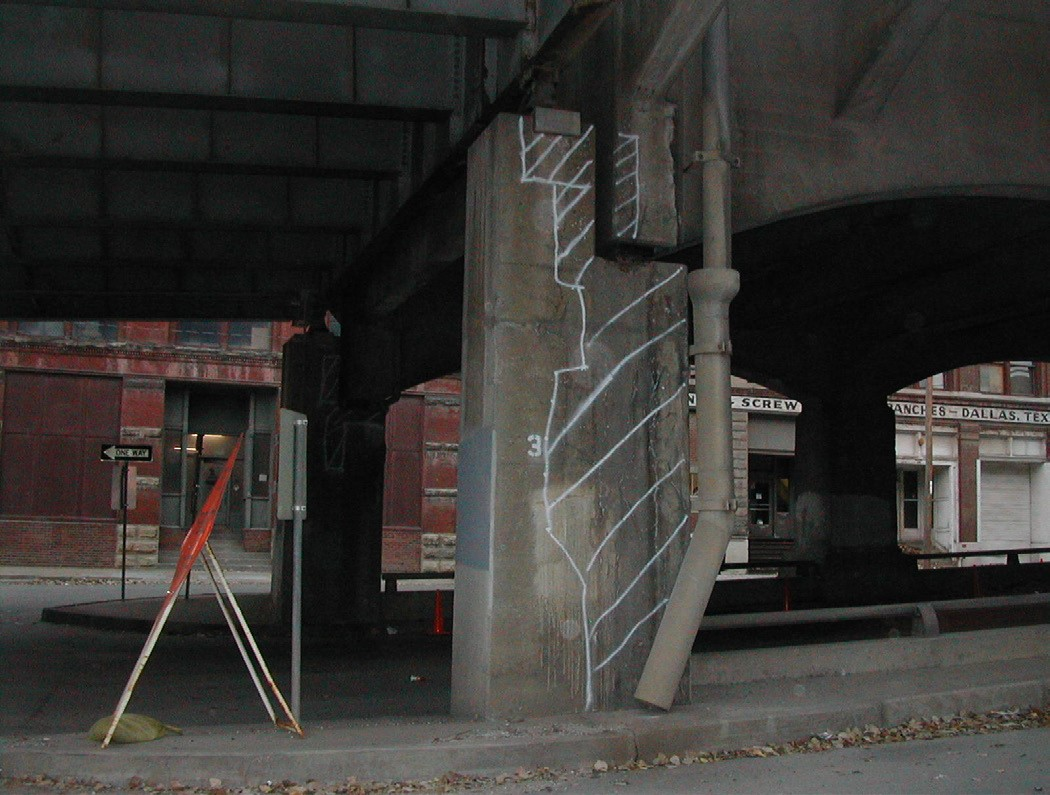
\includegraphics[width=0.6\linewidth]{corrosion-induced-delamination.jpg}
  % \caption{Corrosion-induced delamination on a bridge pier}
  \caption{Corrosion-induced delamination on a bridge pier}
  \label{fig:corrosion-induced-delamination}
\end{figure}

Numerous factors may influence the durability of concrete including water-cement ratio, permeability, curing, shrinkage and cracking, ingredients including admixtures, and the severity of environmental exposure. Due to the high alkalinity of the concrete pore water solution, a thin passive oxide layer is formed and maintained on the surface of the embedded steel thus, protecting it from corrosion activity. Until this passive film is destroyed by the intrusion of aggressive elements or a reduction in the alkalinity of the concrete, the reinforcement will remain in a passive, non-corroding state.

The causes of corrosion are summarized in \cref{fig:causes-of-corrosion-steelbar}. Chloride contamination and carbonation are explained in the sections that follow.

\begin{figure}
  % \includegraphics[width=\linewidth]{graphic-file}
  % \caption{Causes of corrosion of steel in concrete}
  \caption{Causes of corrosion of steel in concrete}
  \label{fig:causes-of-corrosion-steelbar}
\end{figure}


\subsection{Chloride Contamination}
Destruction of the protective oxide film on reinforcing steel is most often caused by the presence of elevated levels of chloride ions. The chloride threshold that initiates corrosion is generally considered to be around 1.0 to 1.4 lbs of water soluble Cl- per cubic yard of concrete (at the level of the steel). This chloride threshold varies depending on the pH of the concrete. For example, concrete that has experienced a loss of alkalinity requires less chloride to initiate corrosion. Chloride-induced corrosion, shown in \cref{fig:chloride-induced-corrosion-steelbar}, is common in structures exposed to deicing salts, marine environments, or certain industrial processes. In some cases, sufficient amounts of chlorides capable of causing corrosion have been introduced during construction by the use of chloride-containing admixtures or
contaminated aggregates.

Non-chloride-bearing salts including calcium magnesium acetate, magnesium acetate, and calcium acetate, lower the freezing temperature of water and can be used for ice control.  However, magnesium-bearing solutions cause severe paste deterioration by forming brucite and non-cementitious magnesium silicate hydrate (Lee et al. 2000).  The detrimental effects caused by calcium acetate were much less severe than those containing magnesium, but the use of these non-chloride-bearing salts has not gained wide acceptance due to cost and the distress they cause.

\begin{figure}
  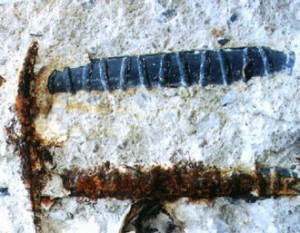
\includegraphics[width=0.6\linewidth]{chloride-induced-corrosion-steelbar.jpg}
  % \caption{Chloride-induced corrosion of reinforcing steel}
  \caption{Chloride-induced corrosion of reinforcing steel}
  \label{fig:chloride-induced-corrosion-steelbar}
\end{figure}
\subsection{Carbonation}
The passive condition of the reinforcing can also be disrupted by the loss of alkalinity in the concrete matrix surrounding the reinforcing steel. It is generally accepted that a pH greater than 10 is sufficient to provide corrosion protection in chloride-free concrete. The reduction in alkalinity is generally caused by carbonation, a reaction between atmospheric carbon dioxide and calcium hydroxide in the cement paste in the presence of water. The result is a reversion of the calcium hydroxide to calcium carbonate (approx. pH 8.5) which has insufficient alkalinity to maintain the passive oxide layer.

The zone of carbonation begins on the surface of atmospherically exposed concrete. The amount of time for the carbonation zone to reach the level of the reinforcing is a function of the thickness of concrete cover, presence and extent of cracks, concrete porosity, humidity levels, and the level of exposure to carbon dioxide.  Carbonation- induced corrosion is more likely to be observed in structures situated in industrial environments where airborne pollutants are commonplace, or in old or historic structures, structures with a high degree of concrete porosity, or structures with low concrete cover over the reinforcement.

In bridge structures, there is generally good quality concrete cover of sufficient thickness (about 2.5 in. in decks) to resist carbonation for up to 100 years.

\section{Strategies for Addressing Corrosion}
\label{sec:strategy-address-corrosion}
Because of the magnitude of the corrosion problem, both the public and private sectors have ongoing activities aimed at reducing or eliminating corrosion damage to concrete structures. While many technologies and materials have been developed for prevention and repair of corrosion-induced damage, the challenge is to select durable, cost- effective technologies and materials from the numerous choices available.

Durability and desired service life must be considered during design. In the case of new structures, it is desirable to avoid, prevent, or delay the initiation of corrosion through the use of low permeability concretes, proper precautions against cracking (see \cref{chp:materials}), and other corrosion-prevention techniques. For existing structures, the condition of the structure should be evaluated to determine if it is corroding or not. If the structure is corroding and the chloride content is high in the concrete, the contaminated concrete is removed; if rust is forming on the surface of the reinforcement, it is cleaned or removed and overlaid with a low permeability concrete overlay. If the existing structure is not corroding, some of the techniques used on new structures, such as applying sealers and membranes, may also be used on the existing structure.

An overview of the available options is provided in \cref{fig:reduced-service-life,fig:options-avoid-corrosion,fig:options-prevent-corrosion,fig:electro-chemical-passivation}.

\begin{figure}
  % \includegraphics[width=\linewidth]{graphic-file}
  % \caption{Reduced service life of reinforced concrete.}
  \caption{Reduced service life of reinforced concrete.}
  \label{fig:reduced-service-life}
\end{figure}

\begin{figure}
  % \includegraphics[width=\linewidth]{graphic-file}
  % \caption{Options for avoiding corrosion}
  \caption{Options for avoiding corrosion}
  \label{fig:options-avoid-corrosion}
\end{figure}

\begin{figure}
  % \includegraphics[width=\linewidth]{graphic-file}
  % \caption{Options for preventing or delaying corrosion initiation.}
  \caption{Options for preventing or delaying corrosion initiation.}
  \label{fig:options-prevent-corrosion}
\end{figure}

\begin{figure}
  % \includegraphics[width=\linewidth]{graphic-file}
  % \caption{Electro-chemical passivation.}
  \caption{Electro-chemical passivation.}
  \label{fig:electro-chemical-passivation}
\end{figure}

Many strategies have been used successfully to improve the corrosion resistance and durability of new structures. These include:
\begin{itemize}
  \item The use of low permeability concrete,
  \item The use of increased concrete cover,
  \item The use of improved construction methods such as curing to minimize cracking,
  \item The use of corrosion-resistant reinforcement,
  \item The use of corrosion inhibitors to increase the corrosion initiation threshold,
  \item The use of membranes, coatings, and sealers, and
  \item The use of improved design details to keep elements dry and to prevent exposure to chlorides.
\end{itemize}

In the United States, epoxy-coated reinforcement (ECR) has been widely used as a corrosion protection system for concrete bridges. However, recent work and observations in the field have shown that the longevity desired (75 years and beyond) may not be achievable and therefore, other corrosion resistant reinforcements are being considered (see \cref{chp:materials} on materials).

Each of these methods can be effective if it significantly extends the time for corrosion to initiate. In many cases it is preferable to employ more than one technique as this will generally reduce the overall risk of corrosion.

Additional information on these topics is provided in \cref{chp:materials} on materials.

\subsection{Existing Structures}
Options for protecting structures from corrosion and extending their service life are much more limited when
dealing with existing structures, as many of the physical parameters are already defined and therefore cannot be
changed or easily altered. In particular, the concrete and reinforcing steel of existing structures are already in place and the characteristics of these materials, including type, quality, cover thickness, permeability, resistance to
corrosion initiation, presence of cracks, etc., are already fixed. Due to these limitations, many of the options that are
viable for new (non-corroding) construction, as shown in \cref{fig:non-corroding-structures}, are not possible or may not be economically
practical for use with existing (corroding) structures. \cref{fig:options-corrod-structures} shows the options for corroding structures.

Despite the reduced number of options available for existing structures, it is still beneficial to be as proactive as
possible. Preventing or delaying corrosion is generally preferable to managing corrosion after it has initiated.
Additional options (and often more economical options) exist to prevent or delay corrosion activity if the structure is
not chloride contaminated or has not already started to corrode.

\begin{figure}
  % \includegraphics[width=\linewidth]{graphic-file}
  % \caption{ Non-corroding structures}
  \caption{Non-corroding structures}
  \label{fig:non-corroding-structures}
\end{figure}

\begin{figure}
  % \includegraphics[width=\linewidth]{graphic-file}
  % \caption{Options for corroding structures.}
  \caption{Options for corroding structures}
  \label{fig:options-corrod-structures}
\end{figure}

\subsection{Levels of Corrosion Protection for Existing Structures}
\subsubsection{Selecting an Active Corrosion Protection Strategy for Reinforced Concrete Structures}
The selection of the appropriate level of corrosion protection is based on many factors such as the level of chloride contamination and carbonation, amount of concrete damage, location of corrosion activity (localized or widespread), the cost and design life of the corrosion protection system, and the expected service life of the structure.

The levels of corrosion protection described in this section are summarized in \cref{tab:levels-corrosion-protection-electrochemical}.

\begin{table}
  % \caption{Summary of the Levels of Corrosion Protection for Electrochemical Corrosion Mitigation Systems.}
  \caption{Summary of the Levels of Corrosion Protection for Electrochemical Corrosion Mitigation Systems.}
  \label{tab:levels-corrosion-protection-electrochemical}
  % \input{tables/levels-corrosion-protection-electrochemical}
\end{table}

\subsubsection{Cathodic Protection}
Cathodic protection provides proven corrosion protection and is intended to effectively stop ongoing corrosion activity. It should be selected when the highest level of protection is necessary and the cost is economically justified.  Cathodic protection systems are grouped into two general categories: impressed current (ICCP) and galvanic (GCP).

Impressed current systems may use titanium or zinc-based anodes and utilize an outside power source. For long- term performance, these systems should be monitored and maintained. Discrete anodes are ideal to protect heavily reinforced concrete, thick structural sections such as columns or beams, or steel framed masonry buildings while titanium ribbon or mesh anodes are placed into slots cut into the concrete surface or cast into a concrete overlay.

Galvanic systems may be designed to provide corrosion control or cathodic protection. These galvanic systems are self-powered and typically require less monitoring and maintenance than ICCP systems. Galvanic jackets are used to protect marine pilings and other structures. Galvanic anodes may be arc-sprayed zinc or otherwise applied to the concrete surface, or they may be cast into a concrete overlay, jacket, or encasement to provide galvanic cathodic protection over a desired area. If galvanic anode systems are cast into concrete or are not directly exposed to a marine environment, they should be activated to ensure that sufficient current is supplied to the reinforcing steel to
provide long lasting corrosion protection.

Cathodic protection systems are generally designed to meet National Association of Corrosion Engineers (NACE) cathodic protection standards and typically use 100mV depolarization as the acceptance criteria (NACE 2000). The current density required to achieve cathodic protection is higher than the current required for corrosion prevention or corrosion control applications. Typical cathodic protection systems operate in the range of 2 to 20 mA/m2 of steel surface area. At these current densities and polarization levels, cathodic protection has demonstrated a very high level of corrosion protection.

Galvanic cathodic protection systems were evaluated in the research phase of the SHRP 2 R19A Project, the report for which is forthcoming. In this study, different galvanic anodes were evaluated for the purpose of minimizing corrosion in reinforced concrete members; a commonly used anode (OA), an anode with 4-times larger zinc surface area than ordinary anodes (OA4), and two high voltage anodes with varying degrees of output voltage (HVAH, higher level; and HVAL, lower level). Concrete test slabs were cast in two layers; the concrete in the upper layer was contaminated with salt to accelerate the corrosion activity and the lower layer was not modified. Salt was not added to the concrete in the lower layer. The test results indicated that there was no corrosion in any of the specimens in the given time period. The testing further indicated that specimens with HVAH provided increased corrosion protection by having higher current and generating more negative potential values than the HVAL.  Anodes having 4-times surface area (OA4) provided additional current and corrosion protection than OA anodes. HVAL anodes exhibited current and potential values similar to the OA4 anodes. Both high voltage anodes and OA4 anodes provided higher current and generated more negative potential values, indicating better corrosion protection than OA anodes. Due to time constraints, the tests were terminated without observing corrosion in the specimens.
Further research with an extended time frame is recommended.

\subsubsection{Corrosion Prevention}
Corrosion prevention is used to keep corrosion activity from initiating in contaminated concrete. In concrete repair projects, the removal and replacement of damaged concrete, if completed in accordance with industry guidelines (ICRI 2008), will address the areas with the highest levels of corrosion. However, new corrosion sites are likely to form in the surrounding contaminated concrete which was passive before the repairs. To mitigate new corrosion activity from occurring around concrete repairs or at other interfaces between new and old concrete, such as bridge widening, joint repairs, and slab replacements, a localized corrosion prevention strategy may be employed utilizing embedded galvanic anodes to extend the life of the concrete repairs. Size and spacing of embedded galvanic anodes should be adjusted to suit site conditions, including quantity and existing condition of reinforcing steel, level of chloride contamination, and environmental conditions.

There has been a significant amount of research in the area of corrosion prevention, some of which has indicated that applied current densities as low as 0.5 to 2.0 mA/m2 of steel surface area have been shown to be effective at preventing the initiation of corrosion for concrete with chloride concentrations up to at least ten times the chloride threshold (Pedeferri 1996). Other research has shown beneficial effects of applied currents between 0.25 and 1.0 mA/m2 (Bertolini et al. 1996).


\subsubsection{Corrosion Control}

Corrosion control systems are utilized in instances in which corrosion has initiated but has not yet progressed to the point of causing concrete damage. The use of corrosion control systems will either stop ongoing corrosion activity or provide a significant reduction in the corrosion rate and increased service life for the rehabilitated structure. In many cases, this level of protection can be provided with low incremental cost, as the protection can be targeted at specific areas of contamination or corrosion activity. Galvanic anodes embedded in drilled holes or installed on a grid pattern in a concrete repair or overlay can be used to provide targeted galvanic corrosion control to columns, beams, decks, posttensioned anchorages, and other areas where ongoing corrosion activity threatens the service life or serviceability of the structure. 

The applied current necessary to control active corrosion is significantly higher than the current required for corrosion prevention. Research has indicated that the typical current density to control active corrosion is in the range of 1 to 7 mA/m2 (Davison et al. 2003).

In the study by Davison et al., corrosion control of specimens with very high initial corrosion rates was achieved.  Some polarization of the reinforcing steel will typically occur at these current densities although the level of polarization may be significantly less than the NACE 100mV depolarization criteria for cathodic protection.

There are many situations where the corrosion activity is moderate or is localized in nature such that corrosion control is an appropriate approach since large scale cathodic protection may not be economically justifiable.  Examples of this include localized areas beneath leaking expansion joints, or decks with isolated areas of high corrosion potentials. In these cases, targeting the protection to address the specific contaminated zone, or “hot spot,” rather than the entire structure may make sense from a cost/benefit point of view.


\subsubsection{Corrosion Passivation/Electrochemical Treatments}
Corrosion passivation is provided by electrochemical treatments that are aimed at directly addressing the cause of the corrosion activity. Electrochemical chloride extraction (ECE) is used to address corrosion caused by chlorides in chloride-contaminated structures.  Electrochemical re-alkalization is used to address corrosion resulting from carbonation of the concrete. These systems are installed on the structure, operated for a short duration, then dismantled and removed leaving the structure in a passive condition. Electrochemical treatments provide many of the long-term corrosion mitigation benefits of cathodic protection systems, but without the need for long-term system maintenance and monitoring. Additional information about the implementation and evaluation of the two systems follows.

Electrochemical chloride extraction is an electrochemical treatment in which an electric field is applied between the reinforcement in the concrete and an externally mounted mesh (\cref{fig:schematic-diagram-ece-treatment}). The mesh is embedded in a conductive media, generally a sprayed-on mixture of lime, water, and cellulose fiber.

\begin{figure}
  % \includegraphics[width=\linewidth]{graphic-file}
  % \caption{Schematic diagram showing ECE treatment process.}
  \caption{Schematic diagram showing ECE treatment process.}
  \label{fig:schematic-diagram-ece-treatment}
\end{figure}

During treatment, the concrete is kept saturated allowing chlorides to go into solution within the pores of the concrete. The negatively charged chloride ions (\ce{Cl-}) are repelled from the negatively charged rebar and attracted toward the positively charged external electrode mesh as a result of the applied electric field. This process lowers the amount of chloride in the concrete and particularly adjacent to the steel. An ECE treatment generally takes 4 to 8 weeks to complete.

In instances of structures with carbonation-induced corrosion, a different electrochemical treatment process, re- alkalization, can be utilized to increase the pH of the concrete cover. The installation for re-alkalization is essentially the same as for ECE except the conductive media is saturated with an alkaline potassium carbonate solution. The potassium (K+) ions in the alkaline solution are transported into the concrete by the application of the electric field.  A re-alkalization treatment generally takes four to seven days to complete and will not re-carbonate.

Electrochemical treatment was evaluated in the research phase of the SHRP 2 R19A Project with detailed results to be presented in the forthcoming final report. In the SHRP 2 study, corrosion resistant reinforcement and electrochemically treated black bars were evaluated to determine if the chloride threshold levels increased to a level to resist corrosion. Both low and high levels of electrochemical treatment were used. The test matrix included black bars, electrochemically-treated black bars, stainless steel bars, and titanium bars, each subjected to salt solution. Due to time constraints, testing was terminated after a total of 26 cycles consisting of four days of wet cycle and 10 days of dry cycle; a total duration of one year. At termination, only one specimen from a set of three with black bars and electrochemically-treated black bars showed an increase in current or potential values indicative of uncertain corrosion activity. The remaining specimens indicated no corrosion activity. Thus, initial observations indicate that electrochemically-treated black bars may not provide the protection expected of stainless steel or titanium; however, whether or not they provide benefits over the black bars without treatment cannot be concluded from this study due to time constraints. Therefore, further research with an extended time frame is recommended.

\section{Case Studies Addressing Corrosion in Existing Structures}
\label{sec:case-study-addressing-corrosion}
\subsection{Project Overview: Impressed Current Cathodic Protection, Corrosion Control, and Electrochemical Chloride Extraction}
During the summer of 1989 and continuing until 1994, the Ontario Ministry of Transportation (MTO) completed a number of restoration and protection projects on the reinforced concrete piers of the Burlington Skyway, a major viaduct located between Toronto and Niagara Falls, Ontario. This work was monitored by MTO’s Materials and Research Branch. Some of this research was conducted under the original SHRP project and is documented in SHRP-C-620, “Evaluation of Norcure Process for Electrochemical Chloride Removal from Steel-Reinforced Concrete Bridge Components” (Bennet and Schue 1993).

An impressed current cathodic protection (ICCP) system was installed on over 200,000ft2 of reinforced concrete substructure. The system was designed to operate as an ICCP system with an applied current density of 10 mA/m2 (1mA/ft2). After an initial period of operation at the design current density, and due to operational issues, the system was run at an average current density of 1mA/m2 (0.1mA/ft2). As such, instead of being operated at cathodic protection current density (2 – 20mA/m2), the system was effectively operated at a corrosion control current density (1 – 7mA/m2). Due to the low applied current density, much of the area did not meet the 100mV NACE criteria for cathodic protection. Despite operating at approximately 10\% of the intended cathodic protection current density, the system operation did fall within typical corrosion control current densities and experienced a significant reduction in concrete deterioration and damage. Over the study period, concrete delamination within the protected area was reduced by 96\% compared to the rate of deterioration of unprotected concrete piers.

Also in 1989, an electrochemical chloride extraction trial was completed by MTO on a section of the same structure. The treated portion was comprised of rectangular piers and bents. The piers were contaminated with chlorides due to long-term leakage of the deck joints above.

Electrochemical chloride extraction was used to reduce the chloride content of the concrete to below the threshold level of corrosion at the rebar. This process eliminated high corrosion potential readings and corrosion potentials in the treated area were shifted into the passive range as shown in \cref{tab:corrosion-potential-measurements}; in this table ECE treated section exhibited a high percentage of area with a low risk of corrosion. Corrosion current as measured by linear polarization (3-LP) was greatly reduced as shown in \cref{tab:corrosion-current-measurements}; in this table ECE treated sections exhibited a high percentage of passive area. Thus, corrosion potentials and corrosion currents were reduced to the passive, noncorroding range as a result of the electrochemical chloride extraction treatment for a 20-year duration as shown in \cref{tab:corrosion-potential-measurements,tab:corrosion-current-measurements}. These readings have remained stable and show no significant changes over the period.

Additional piers were treated during the fall of 1997 as part of the next phase of work on this project. The longterm results from these more recent tests are expected to be similar to the electrochemical chloride extraction trial completed in 1989.

\begin{table}
  \caption{Corrosion Potential Measurements}
  \label{tab:corrosion-potential-measurements}
  % \input{tables/filename}
\end{table}

\begin{table}
  \caption{Corrosion Current Measurements}
  \label{tab:corrosion-current-measurements}
  % \input{tables/filename}
\end{table}

\subsection{Project Overview: Galvanic Cathodic Protection: Galvanic Encasement of Severely Corroded Elements}

Galvanic anodes have also been developed for more global corrosion control. One such configuration is the system installed to repair and protect severely damaged and corroding bridge abutments in the Midwest (\cref{fig:distribute-anode}). The abutments had been contaminated with chlorides causing corrosion of the reinforcing steel and significant concrete damage.

\begin{figure}
  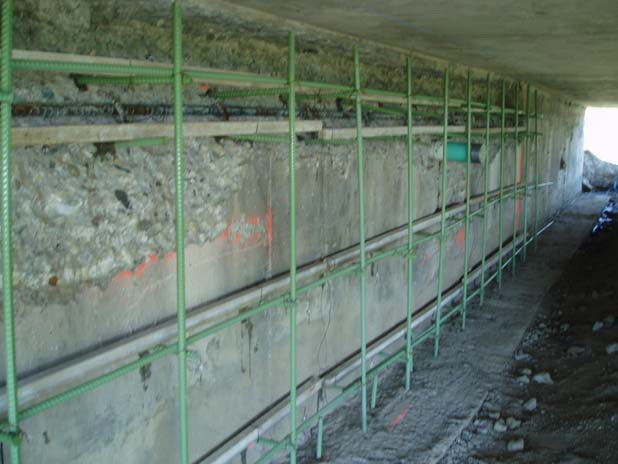
\includegraphics[width=0.6\linewidth]{distribute-anode.jpg}
  % \caption{A distributed anode system used for corrosion control bridge abutment in the Midwest.}
  \caption{A distributed anode system used for corrosion control bridge abutment in the Midwest.}
  \label{fig:distribute-anode}
\end{figure}

As part of the rehabilitation, which also included enlargement and strengthening of the abutment, the cracked and spalled concrete was removed. \cref{fig:abutment-section-rehabilitation} shows the cross-sectional detail of the rehabilitation system. Elongated anodes were connected to the existing reinforcing steel and encased in a new layer of concrete to reface the abutment wall. The purpose of the anodes was to protect the existing steel from chloride-induced corrosion. This allowed uncracked chloride-contaminated concrete to remain in place, and thereby reduce concrete breakout and the need for structural shoring. The cross-sectional configuration of the repaired abutment wall and adjoining structural elements is shown in \cref{fig:abutment-section-rehabilitation}.

\begin{figure}
  % \includegraphics[width=\linewidth]{graphic-file}
  \caption{Cross-sectional detail of the abutment rehabilitation system.}\label{fig:abutment-section-rehabilitation}
\end{figure}

The current output, shown in {fig:current-output}, appears to be strongly related to temperature. Its magnitude varied considerably with temperature on an annual basis, with the mean current density gradually reducing year by year. After supplying an initial current of over 35 mA/m2 of steel area in the first few days, it averaged over 8 mA/m2 during the first year, lowering gradually to around 5 mA/m2 in the fourth year. These levels of current density are within the design limits of 2 to 20 mA/m2 of steel area for cathodic protection as specified in BS EN 12696:2012 (BS 2012). Current densities in impressed current cathodic protection systems are also normally reduced with age as the steel becomes easier to polarize. Depolarization levels were measured to be well in excess of 100mV as specified in the same standard, suggesting that the galvanic system was deemed to satisfy the criteria for cathodic protection of steel reinforcement. Depolarization and corrosion protection status are given in \cref{tab:corrosion-protection-status}.

\begin{figure}
  % \includegraphics[width=\linewidth]{graphic-file}
  \caption{Current output of anode system and its relationship to temperature.}\label{fig:current-output}
\end{figure}

\begin{table}
  \caption{Depolarization and Corrosion Protection Status}\label{tab:corrosion-protection-status}
  % \input{tables/filename}
\end{table}


\subsection{Project Overview: Corrosion Prevention Using Galvanic Anodes}
The oldest site trial of discrete galvanic anodes is over 10 years old (\cref{fig:bridge-north-side}). To verify the performance of the anodes, 12 anodes were installed in an otherwise conventional patch repair on the soffit of a bridge beam (\cref{fig:installation-anodes}). The performance of these anodes was monitored with time.

\begin{figure}
  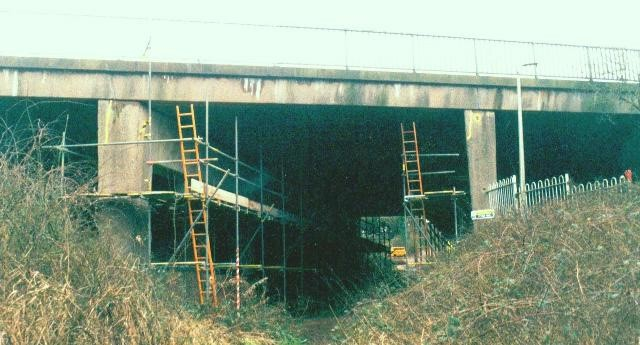
\includegraphics[width=0.8\linewidth]{bridge-north-side.jpg}
  % \caption{North side of bridge.}
  \caption{North side of bridge.}
  \label{fig:bridge-north-side}
\end{figure}
\begin{figure}
  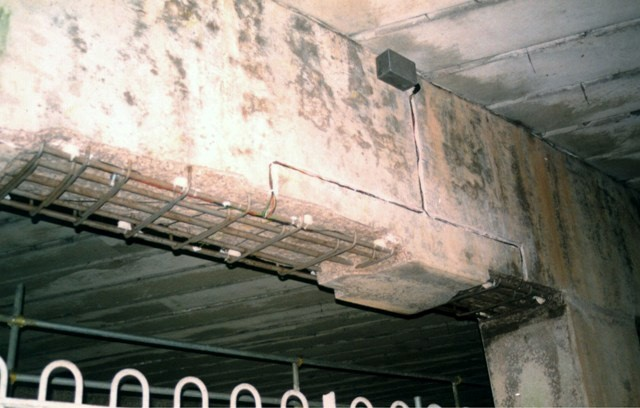
\includegraphics[width=0.8\linewidth]{installation-anodes.jpg}
  % \caption{Installation of anodes within the repaired area of a beam also showing control box and wiring.}
  \caption{Installation of anodes within the repaired area of a beam also showing control box and wiring.}
  \label{fig:installation-anodes}
\end{figure}

The anodes were inserted around the perimeter of the repair area between 600mm and 700mm centers (\cref{fig:installation-anodes}). The anodes were installed to enable monitoring by connecting a single wire from each anode to a control box such that the anodes could be monitored via the box. Monitoring of the anodes consisted of measuring current output for each installed anode, and, on occasion, performing a depolarization test over a 4-hour or 24-hour period after disconnection of the anodes. Monitoring started in April 1999.


\subsection{Results and Discussion}
The 10-year results of the current output of each anode are presented in \cref{fig:protective-current}. They indicate a variable current depending on the ambient temperature and moisture content in the concrete. For example, the same anode could generate up to 400-600μA of current during hot periods and less than 100μA during cold spells. Corrosion of the steel is expected to have similarly-varying corrosion rates so that the current output of the anodes is thought to be self-regulating, producing higher levels when the steel is corroding most.

\begin{figure}
  % \includegraphics[width=\linewidth]{graphic-file}
  \caption{Protective current from galvanic anodes over a 10-year period.}\label{fig:protective-current}
\end{figure}

Systems such as this are designed to prevent the onset of corrosion of the reinforcement. The current density required for corrosion prevention (referred to as cathodic prevention in Europe) is 0.2-2mA/m2, as reported by Bertolini et al. (1993) and Pedeferri (1996), and adapted in the European Standard BS EN 12696:2012 (BS 2012). Based on the steel surface area within the repaired and affected adjacent area, the mean current density ranged between \qty{0.6}{mA/m^2} and \qty{3.0}{mA/m^2} through the duration of this trial, with a mean current density of around \qty{1.4}{mA/m^2} over the 10-year period. This current density is within the suggested range of \qtyrange{0.2}{2.0}{mA/m^2} for corrosion prevention (cathodic prevention).

Monitoring the depolarized potential of the steel in the vicinity of the repair with time may be another way of determining the effectiveness of the system. \cref{fig:depolarize-potentials-with-time}, which shows the mean depolarized potential with time both within and outside of the repaired area, indicates that the mean potential is moving to a more noble level with time. This indicates increasing passivation of the steel over time.

\begin{figure}
  % \includegraphics[width=\linewidth]{graphic-file}
  \caption{Mean depolarized steel potentials with time (4 hours or 24 hours after disconnection of the anodes).}\label{fig:depolarize-potentials-with-time}
\end{figure}